
\documentclass{beamer}
\usetheme{Copenhagen}
%https://en.wikibooks.org/wiki/LaTeX/Macros
\usepackage{tikz}
%vectors, matrices, complex numbers,  trigonometrie, big O notation, grafentheorie, vertaling van probleem in algoritme,
\useoutertheme{infolines}

\newcommand{\drawcgridaxes}{
\draw[step=1cm,gray,very thin] (-3,-3) grid (3,3);
\draw[thick,->] (0,0) -- (3,0) node[right] {real};
\draw[thick,->] (0,0) -- (0,3) node[above] {imaginary};
\draw[thick,->] (0,0) -- (-3,0);
\draw[thick,->] (0,0) -- (0,-3);
}

\newcommand{\drawgridaxes}{
\draw[step=1cm,gray,very thin] (-3,-3) grid (3,3);
\draw[thick,->] (0,0) -- (3,0) node[anchor=north west] {x};
\draw[thick,->] (0,0) -- (0,3) node[anchor=south east] {y};
\draw[thick,->] (0,0) -- (-3,0);
\draw[thick,->] (0,0) -- (0,-3);
}

\newcommand{\drawtdvec}[2]{
\begin{tikzpicture}[scale=0.70]
\drawgridaxes
\draw[red, thick, ->] (0,0) -- (#1,#2);
\end{tikzpicture}
}

\newcommand{\drawbasicvec}{
		\begin{equation*} \vec{V} = \begin{bmatrix} 1 \\ 2 \end{bmatrix} \end{equation*}

        \drawtdvec{1}{2}
}

\newcommand{\tcframe}[3] {
	\frame {
		\frametitle{#1}
\begin{columns}
\begin{column}{0.5\textwidth}
		#2
\end{column}

\begin{column}{0.5\textwidth}
		#3
\end{column}
\end{columns}
}
}

\definecolor{darkgreen}{RGB}{0,150,0}


\title{Vizualizing math}
\subtitle{Using math for pictures, using pictures to explain the math.}

\begin{document}
	\frame {
		\titlepage
	}
	
	\frame {
		\frametitle{Drawing on your computer}
		\includegraphics{face}
	}
	
	\tcframe{The color of a pixel}
		{\includegraphics[width=1\columnwidth]{pixel_code}}
		{\includegraphics[width=1\columnwidth]{pixel}}

	\tcframe{Let the computer do graphics}
		{\includegraphics[width=1\columnwidth]{random_pixels_code.png}}
		{\includegraphics[width=1\columnwidth]{random_pixels.png}}
	
	\tcframe{What am I looking at}
		{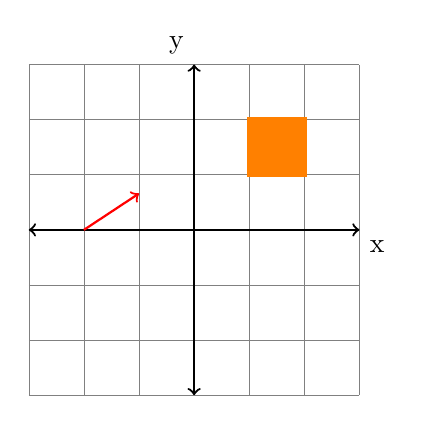
\begin{tikzpicture}[scale=0.70]
        \drawgridaxes
        \draw[red, thick, ->] (-2,0) -- (-1,0.66);
        \draw[orange, ultra thick, fill=orange] (1,1) rectangle (2,2);
        \end{tikzpicture}
        }
        {\includegraphics[width=1\columnwidth]{orange_square}}
        
	
	\tcframe{Vector, representation}
	{\drawbasicvec}
    {\includegraphics[width=1\columnwidth]{basic_vector_code.png}}
	
	\tcframe{Scaling a vector}
	{\drawbasicvec}
	{\begin{equation*} 1.5 * \vec{V} = \begin{bmatrix} 1.5 \\ 3  \end{bmatrix} \end{equation*}
		\drawtdvec{1.5}{3}}
		
	\frame {
		\frametitle{Code for scaling a vector}
		\includegraphics[width=1\columnwidth]{scale_code}
	}
		
	\tcframe{Scaling with negative number}
	{\drawbasicvec}
	{\begin{equation*} -1.5 * \vec{V} = \begin{bmatrix} -1.5 \\ -3  \end{bmatrix} \end{equation*}
		\drawtdvec{-1.5}{-3}}
	
	\tcframe {Scaling all happens on the same line}
		{
		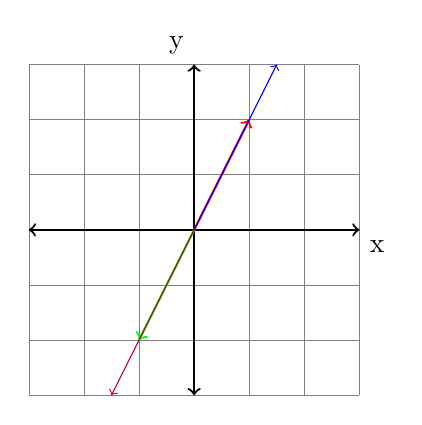
\begin{tikzpicture}[scale=0.70]
        \drawgridaxes
        \draw[red, thick, ->] (0,0) -- (1,2);
        \draw[green, thick, ->] (0,0) -- (-1,-2);
        \draw[blue, ->] (0,0) -- (1.5,3);
        \draw[purple, ->] (0,0) -- (-1.5,-3);
        \end{tikzpicture}
        }
        {
        \begin{equation*} t * \vec{v}
        \end{equation*}
        }
	
	
	\frame {
		\frametitle{Adding vectors, or splitting up in components}
		\begin{equation*} \begin{bmatrix} 2 \\ 0 \end{bmatrix} + \begin{bmatrix} 0 \\ 1 \end{bmatrix} = \begin{bmatrix} 2 \\ 1 \end{bmatrix}\end{equation*}
		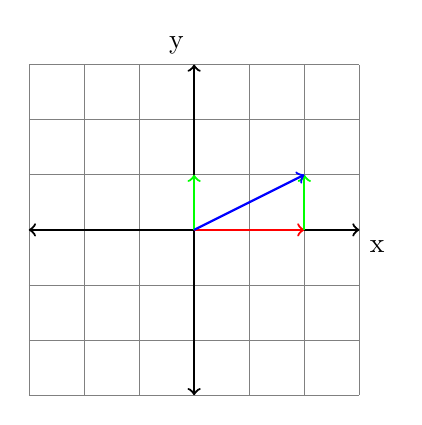
\begin{tikzpicture}[scale=0.70]
        \drawgridaxes
        \draw[red, thick, ->] (0,0) -- (2,0);
        \draw[green, thick, ->] (0,0) -- (0,1);
        \draw[green, thick, ->] (2,0) -- (2,1);
        \draw[blue, thick, ->] (0,0) -- (2,1);
        \end{tikzpicture}
	}
	
	\frame {
		\frametitle{Code for adding vectors}
		\includegraphics{add_vectors_code.png}
	}
	
	\frame {
		\frametitle{Subtracting vectors}
		\begin{equation*} \begin{bmatrix} 2 \\ 1 \end{bmatrix} - \begin{bmatrix} 2 \\ 0 \end{bmatrix} = \begin{bmatrix} 0 \\ 1 \end{bmatrix}\end{equation*}
		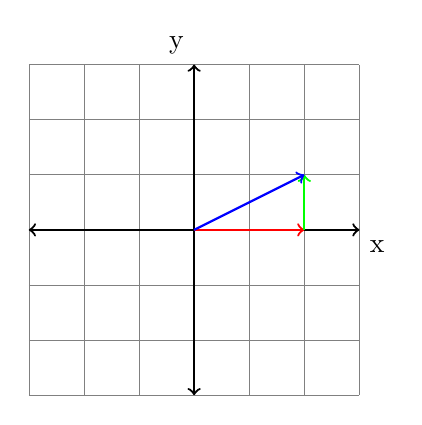
\begin{tikzpicture}[scale=0.70]
        \drawgridaxes
        \draw[red, thick, ->] (0,0) -- (2,0);
        \draw[green, thick, ->] (2,0) -- (2,1);
        \draw[blue, thick, ->] (0,0) -- (2,1);
        \end{tikzpicture}
	}
	
	\tcframe
	{Inner product}
	{
		\begin{equation*} \begin{bmatrix} 2 \\ 1 \end{bmatrix} \cdot \begin{bmatrix} 3 \\ 4 \end{bmatrix} = 2*3 + 1 * 4\end{equation*}
		\begin{equation*} \vec{c}^2 = \begin{bmatrix} a \\ b \end{bmatrix} \cdot \begin{bmatrix} a \\ b \end{bmatrix} = a*a + b*b\end{equation*}
		\begin{block}{}
			\begin{equation*} a^2 + b^2 = c^2\end{equation*}
		\end{block}
		}
		{
		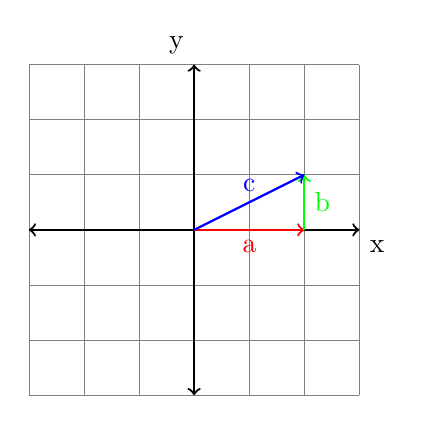
\begin{tikzpicture}[scale=0.70]
        \drawgridaxes
        \draw[red, thick, ->] (0,0) -- (2,0) node[midway, below] {a};
        \draw[green, thick, ->] (2,0) -- (2,1) node[midway, right] {b};
        \draw[blue, thick, ->] (0,0) -- (2,1) node[midway, above] {c};
        \end{tikzpicture}
	}
	
		\frame {
		\frametitle{Inner product, projection}
		\begin{equation*} \begin{bmatrix} 1 \\ 0 \end{bmatrix} \cdot \begin{bmatrix} 2 \\ 1 \end{bmatrix} = 1*2 + 0 * 1 = 2 \end{equation*}
		\begin{equation*} \begin{bmatrix} 0 \\ 1 \end{bmatrix} \cdot \begin{bmatrix} 2 \\ 1 \end{bmatrix} = 0*2 + 1*1 = 1 \end{equation*}
		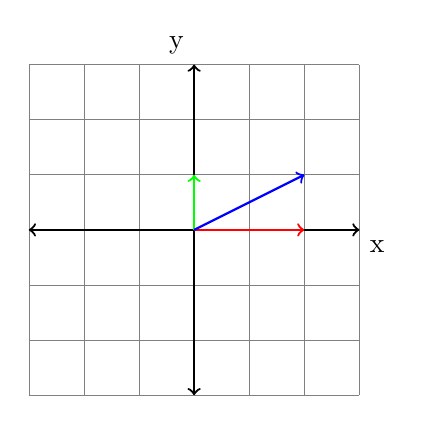
\begin{tikzpicture}[scale=0.70]
        \drawgridaxes
        \draw[red, thick, ->] (0,0) -- (2,0);
        \draw[green, thick, ->] (0,0) -- (0,1);
        \draw[blue, thick, ->] (0,0) -- (2,1);
        \end{tikzpicture}
	}
	
	\frame {
		\frametitle{Code for inner product}
		\includegraphics{inner_product_code.png}
	}
	
	\frame {
		\frametitle{Vectored}
		\includegraphics{You_Just_Got_Vectored.jpg}
	}
	
	\frame{
	    \frametitle{Movement}
	    \begin{center}
		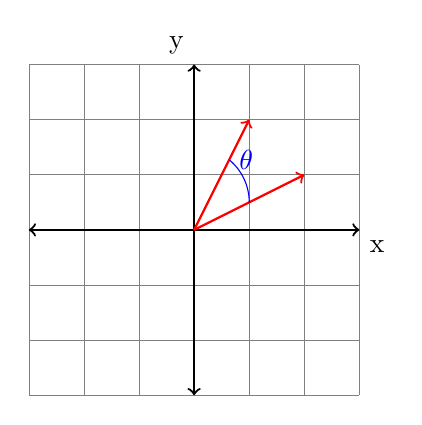
\begin{tikzpicture}[scale=0.70]
        \drawgridaxes
        \draw[red, thick, ->] (0,0) -- (1,2);
        \draw[red, thick, ->] (0,0) -- (2,1);
        \draw[blue] (1,0.5) arc (0:50:1cm) node[right] {$\theta$};
        \end{tikzpicture}
        \end{center}
        }

	
	\tcframe {Matrix, representation}
		{\begin{equation*} \textbf{M} = \begin{bmatrix} 0.2 & 0.3 \\ 0.5 & 0.6 \end{bmatrix} \end{equation*}}
		{		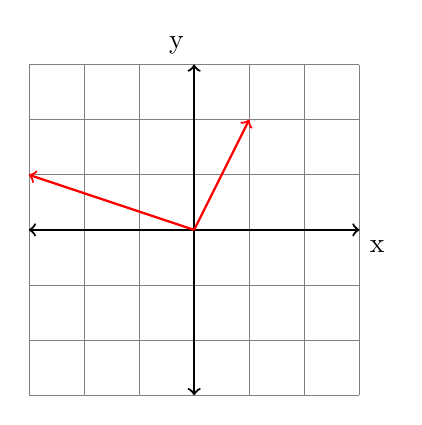
\begin{tikzpicture}[scale=0.70]
        \drawgridaxes
        \draw[red, thick, ->] (0,0) -- (1,2);
        \draw[red, thick, ->] (0,0) -- (-3,1);
        \end{tikzpicture}}
	
	\frame {
		\frametitle{Multiplying matrix with a vector}
		\begin{equation*} \textbf{M} = \begin{bmatrix} a & b \\ c & d \end{bmatrix} * \begin{bmatrix} x \\ y \end{bmatrix} = \begin{bmatrix} a * x + b * y \\ c * x + d * y \end{bmatrix}\end{equation*}
		\begin{center}
		\includegraphics[width=0.7\columnwidth]{matrix_mult_code.png}
		\end{center}
	}
	\frame {
		\frametitle{Identity matrix}
		\begin{equation*} \textbf{M} = \begin{bmatrix} 1 & 0 \\ 0 & 1 \end{bmatrix} * \begin{bmatrix} 2 \\ 3 \end{bmatrix} = \begin{bmatrix} 1 * 2 + 0 * 3 \\ 0 * 2 + 1 * 3 \end{bmatrix} = \begin{bmatrix} 2 \\ 3 \end{bmatrix}\end{equation*}
	}
	\frame {
		\frametitle{90 degrees rotation matrix}
		\begin{equation*} \textbf{M} = \begin{bmatrix} 0 & -1 \\ 1 & 0 \end{bmatrix} * \begin{bmatrix} 1 \\ 2 \end{bmatrix} = \begin{bmatrix} 0 * 1 + -1 * 2 \\ 1 * 1 + 0 * 2 \end{bmatrix} = \begin{bmatrix} -2 \\ 1 \end{bmatrix}\end{equation*}
		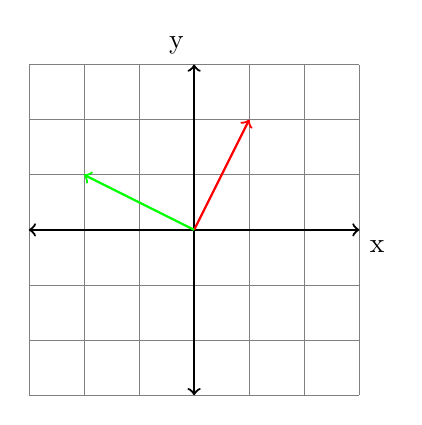
\begin{tikzpicture}[scale=0.70]
        \drawgridaxes
        \draw[red, thick, ->] (0,0) -- (1,2);
        \draw[green, thick, ->] (0,0) -- (-2,1);
        \end{tikzpicture}
	}
	\tcframe {Sin and Cos, rotation from x-axis}
		{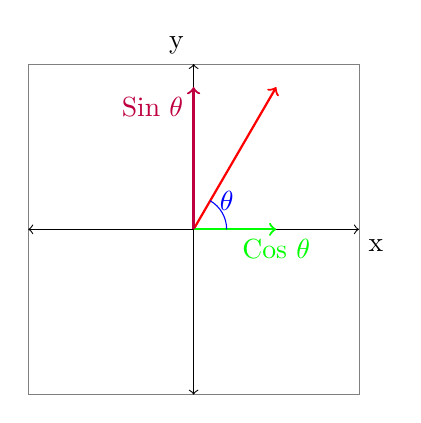
\begin{tikzpicture}[scale=2.10]
		\draw[step=1cm,gray,very thin] (-1,-1) grid (1,1);
        \draw[thin,->] (0,0) -- (1,0) node[anchor=north west] {x};
        \draw[thin,->] (0,0) -- (0,1) node[anchor=south east] {y};
        \draw[thin,->] (0,0) -- (-1,0);
        \draw[thin,->] (0,0) -- (0,-1);
        \draw[red, thick, ->] (0,0) -- (0.5,0.86);
        \draw[green, thick, ->] (0,0) -- (0.5,0) node[below] {Cos $\theta$};
        \draw[purple, thick, ->] (0,0) -- (0,0.86) node[anchor=north east] {Sin $\theta$};
        \draw[blue] (0.2,0) arc (0:60:0.2cm) node[right] {$\theta$};
        \end{tikzpicture}}
	    {
	    \begin{equation*} \textbf{M} = \begin{bmatrix} \cos(\theta) & 0 \\ \sin(\theta) & 0 \end{bmatrix} * \begin{bmatrix} 1 \\ 0 \end{bmatrix} = \begin{bmatrix} \cos(\theta) \\ \sin(\theta) \end{bmatrix}\end{equation*}
	    }
	    
	   \tcframe {Sin and Cos, rotation from y-axis}
		{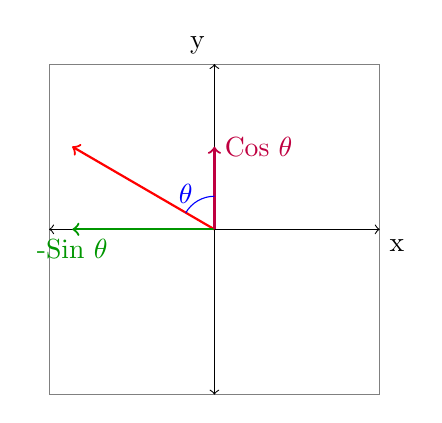
\begin{tikzpicture}[scale=2.10]
		\draw[step=1cm,gray,very thin] (-1,-1) grid (1,1);
        \draw[thin,->] (0,0) -- (1,0) node[anchor=north west] {x};
        \draw[thin,->] (0,0) -- (0,1) node[anchor=south east] {y};
        \draw[thin,->] (0,0) -- (-1,0);
        \draw[thin,->] (0,0) -- (0,-1);
        \draw[red, thick, ->] (0,0) -- (-0.86,0.5);
        \draw[darkgreen, thick, ->] (0,0) -- (-0.86,0) node[below] {-Sin $\theta$};
        \draw[purple, thick, ->] (0,0) -- (0,0.5) node[right] {Cos $\theta$};
        \draw[blue] (0,0.2) arc (90:150:0.2cm) node[above] {$\theta$};
        \end{tikzpicture}}
	    {
	    \begin{equation*} \textbf{M} = \begin{bmatrix} 0 & -\sin(\theta) \\ 0 & \cos(\theta) \end{bmatrix} * \begin{bmatrix} 0 \\ 1 \end{bmatrix} = \begin{bmatrix} -\sin(\theta) \\ \cos(\theta) \end{bmatrix}\end{equation*}
	    }
	    
	\frame {
		\frametitle{Rotation matrix}
		\begin{equation*} \begin{bmatrix} \cos(\theta) & -\sin(\theta) \\ \sin(\theta) & \cos( \theta) \end{bmatrix}
		\end{equation*}
	}
	
	%-----------------------------------------ABC----------------------------------------------------
	
	\tcframe{Do we hit the orange}
		{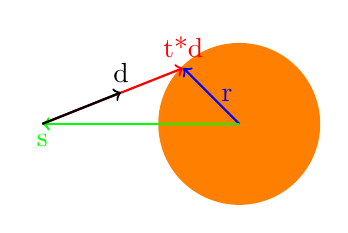
\begin{tikzpicture}[scale=1]
        \draw[orange, ultra thick, fill=orange] (0,0) circle (1);
        \draw[red, thick, ->] (-2.5,0) -- (-0.71,0.71) node[above] {t*d};
        \draw[blue, thick, ->] (0,0) -- (-0.71,0.71) node[midway, right] {r};
        \draw[green, thick, ->] (0,0) -- (-2.5,0) node[below] {s};
        \draw[black, thick, ->] (-2.5,0) -- (-1.5,0.4) node[above] {d};
        \end{tikzpicture}
        }
        {		
        \begin{block}{}
        \begin{equation*} (a + b)^2 = a^2 + b^2 + 2*a*b\end{equation*}
        \end{block}
		\begin{equation*} (\vec{s} + t * \vec{d})^2 = r^2
		\end{equation*}
		\begin{equation*}  t^2 * \vec{d}^2 + t * 2(\vec{s} \cdot \vec{d}) + \vec{s}^2 - r^2 = 0
		\end{equation*}
		}

	\frame {
	    \frametitle{Quadratic formula}
	   \begin{block}{}
		\begin{equation*} t^2*a + t*b + c = 0
		\end{equation*}
		\end{block}
	    
	    \begin{block}{}
		\[t = \frac{-b \pm \sqrt{b^2 - 4 a c}}{2a}\]
		\end{block}
		
		\begin{alertblock}{}
		\begin{equation*} b^2 - 4 a c >= 0
		\end{equation*}
		\end{alertblock}
	}
	
	\frame {
	    \frametitle{Quadratic formula}
	    \begin{equation*}  t^2 * \vec{d}^2 + t * 2(\vec{s} \cdot \vec{d}) + \vec{s}^2 - r^2 = 0
		\end{equation*}
				\begin{equation*} a = \vec{d}^2
		\end{equation*}
				\begin{equation*} b = 2(\vec{s} \cdot \vec{d})
		\end{equation*}
				\begin{equation*} c = \vec{s}^2 - r^2
		\end{equation*}

		\begin{alertblock}{}
		\begin{equation*} b^2 - 4 a c >= 0
		\end{equation*}
		\end{alertblock}
	}
	
		\frame {
		\frametitle{Code for hitting the circle}
		\includegraphics[width=1\columnwidth]{hitting_the_circle_code.png}
	}
	
		\frame {
		\frametitle{Result of hitting the circle}
		\includegraphics[width=0.4\columnwidth]{hitting_the_circle_result.png}
	}
	
	\frame {
		\frametitle{3D version}
		\includegraphics[width=1\columnwidth]{minirt_mandatory.png}
	}
	
	\frame {
		\frametitle{And then...}
		\includegraphics[width=1\columnwidth]{miniRT}
	}
	
	\tcframe{Complex numbers}
		{\begin{equation*} c = a + bi
		\end{equation*}
	    \begin{equation*} i^2 = -1
		\end{equation*}
	}
	{
	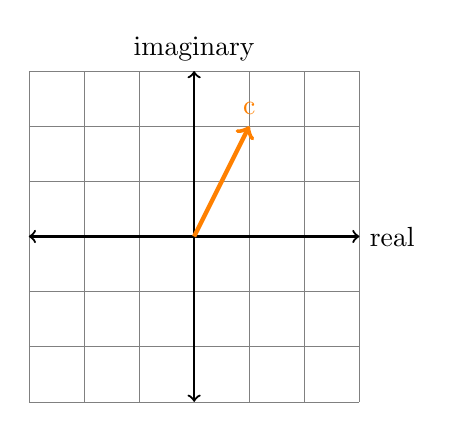
\begin{tikzpicture}[scale=0.70]
	\drawcgridaxes
	\draw[orange, ultra thick, ->] (0,0) -- (1,2) node[above] {c};
	\end{tikzpicture}
	}
	
	\tcframe{Adding complex numbers}
		{\begin{equation*} (0 + 2i) + (2 + 1i) = 2 + 3i  
		\end{equation*}
	}
	{
	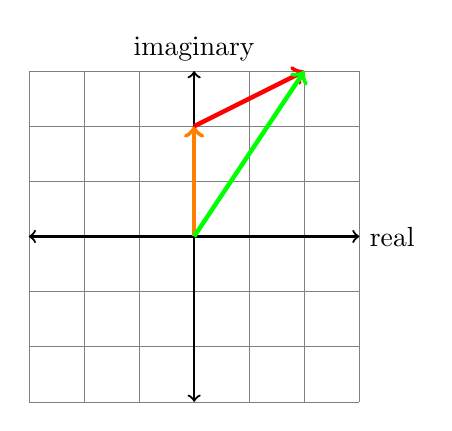
\begin{tikzpicture}[scale=0.70]
	\drawcgridaxes
	\draw[orange, ultra thick, ->] (0,0) -- (0,2);
	\draw[red, ultra thick, ->] (0,2) -- (2,3);
	\draw[green, ultra thick, ->] (0,0) -- (2,3);
	\end{tikzpicture}
	}
	
	\frame {
		\frametitle{Code for adding complex numbers}
		\includegraphics[width=1\columnwidth]{cpx_add_code.png}
	}
	
	\frame {
		\frametitle{Multiplying complex numbers}
		\begin{equation*} (a_1 + b_1i) * (a_2 + b_2i) = (a_1 * a_2) + (a_1 * b_2i) + (b_1i * a_2) + (b_1i * b_2i) 
		\end{equation*}
		\begin{equation*}
		= (a_1 * a_2 - b_1 * b_2) + (a_1 * b_2 + b_1 * a_2)i
		\end{equation*}
	}
	
		\frame {
		\frametitle{Code for multiplying complex numbers}
		\includegraphics[width=1\columnwidth]{cpx_multiply_code.png}
	}
	
	\tcframe{Multiplying complex numbers example}
		{\begin{equation*} i * (2 + 1i) = -1 + 2i  
		\end{equation*}
	}
	{
	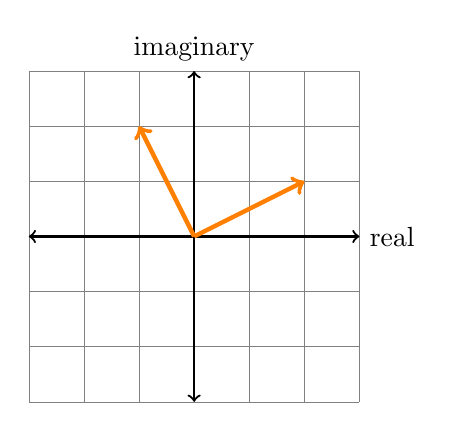
\begin{tikzpicture}[scale=0.70]
	\drawcgridaxes
	\draw[orange, ultra thick, ->] (0,0) -- (2,1);
	\draw[orange, ultra thick, ->] (0,0) -- (-1,2);
	\end{tikzpicture}
	}
	

	

	
	\frame {
		\frametitle{Complex numbers, rotation}
		\begin{equation*} (\cos(\theta) + i*\sin(\theta)) * (a + bi)
		\end{equation*}
		\begin{equation*}
		= \begin{bmatrix} \cos(\theta) & -\sin(\theta) \\ \sin(\theta) & \cos(\theta) \end{bmatrix} * \begin{bmatrix} a \\ b \end{bmatrix}
		\end{equation*}
	}
	
	\frame {
		\frametitle{Code for taking the squared length of complex numbers}
		\includegraphics[width=1\columnwidth]{cpx_ls_code.png}
	}
	
	\frame {
	\frametitle{Julia set, Mandelbrot set}
	\begin{center}
	$z = z^2 + c$
	\end{center}
	}
	
	\frame {
	\frametitle{Mandelbrot}

	\begin{block}{}
		\begin{center}
	$z = z^2 + c$ \\
			\end{center}
	\end{block}

	\begin{block}{}
		\begin{center}
	%$0.5 = 0^2 + 0.5$ \\
	%$0.75 = 0.5^2 + 0.5$ \\
	%$1.0625 = 0.75^2 + 0.5$ \\
	$1 = 0^2 + 1$ \\
	$2 = 1^2 + 1$ \\
	$5 = 2^2 + 1$ \\
		\end{center}
	\end{block}
	
			\begin{block}{}
			\begin{center}

	$0 = 0^2 + 0$ \\

		\end{center}
		\end{block}
	
		\begin{block}{}
			\begin{center}

	$0.25 = 0^2 + 0.25$ \\
	$0.3125 = 0.25^2 + 0.25$ \\
	$0.3477 = 0.3125^2 + 0.25$ \\
	... \\
	$0.25 = 0.5^2 + 0.25$
		\end{center}
		\end{block}

	}
	
	\frame {
		\frametitle{Mandelbrot code}
		\includegraphics[width=1\columnwidth]{mandelbrot code.png}
	}
	
	\frame {
		\frametitle{Mandelbrot result}
		\includegraphics[width=1\columnwidth]{mandelbrot_result.png}
	}
	
	\frame {
		\frametitle{Julia code}
		\includegraphics[width=1\columnwidth]{julia_code.png}
	}
	
	\frame {
		\frametitle{Julia result}
		\includegraphics[width=1\columnwidth]{julia_result.png}
	}
	
	\frame {
		\frametitle{rvan-mee}
		\includegraphics[width=1\columnwidth]{fractol_rvanmee.png}
	}
	
		\frame {
		\frametitle{slides}
		\begin{center}
			https://github.com/GroteGnoom/codam\_presentation
			\end{center}
			}

	
	%https://en.wikipedia.org/wiki/Complex_number#Matrix_representation_of_complex_numbers
\end{document}
